\documentclass[conference]{IEEEtran}
\IEEEoverridecommandlockouts
% The preceding line is only needed to identify funding in the first footnote. If that is unneeded, please comment it out.
\usepackage{cite}
\usepackage{amsmath,amssymb,amsfonts}
\usepackage{algorithmic}
\usepackage{graphicx}
\usepackage{textcomp}
\usepackage{xcolor}

\def\BibTeX{{\rm B\kern-.05em{\sc i\kern-.025em b}\kern-.08em
    T\kern-.1667em\lower.7ex\hbox{E}\kern-.125emX}}
\begin{document}

\title{Documentation of Fresh fruit detection AI}

\author{
\IEEEauthorblockN{1\textsuperscript{st} Bernard Swanepoel}
\IEEEauthorblockA{Faculty of Natural\\
and Agricultural Sciences\\
North-West University\\
39909476\\
Email: 39909476@mynwu.ac.za}
\and
\IEEEauthorblockN{2\textsuperscript{nd} Ashton du Plessis}
\IEEEauthorblockA{Faculty of Natural\\
and Agricultural Sciences\\
North-West University\\
34202676\\
Email: 34202676@mynwu.ac.za}
\and
\IEEEauthorblockN{3\textsuperscript{rd} Nico Deng}
\IEEEauthorblockA{Faculty of Natural\\
and Agricultural Sciences\\
North-West University\\
33700710\\
Email: 33700710@mynwu.ac.za}
}
\maketitle

\begin{abstract}
This paper presents a convolutional neural network (CNN) model and a mobile application for classifying fresh and rotten fruits. The CNN model is designed to distinguish between fresh and rotten apples, bananas, and oranges using image data. The model architecture consists of multiple convolutional layers, batch normalization, dropout, and fully connected layers. The training process utilizes data augmentation techniques, such as random horizontal flipping and normalization, to enhance the model's performance. The model is trained on a dataset of fruit images and evaluated for its classification accuracy. Additionally, a mobile application is developed to integrate the trained model for real-time fruit classification. The application allows users to load fruit images, preprocess them, and obtain predictions from the CNN model. The predicted class, either fresh or rotten fruit, is displayed to the user along with the corresponding image. The proposed system demonstrates the potential for automating fruit quality assessment and facilitating efficient sorting and grading processes in the agricultural industry or daily use.
\\
\end{abstract}

\begin{IEEEkeywords}
Rectified Linear units, Deep Learning,
Neural Networks, Supervised Learning, Structured Learning
\end{IEEEkeywords}

\section{Introduction}

It is known that some people find it difficult to identify whether fruit is fresh or rotten. This can be due to various factors such as visual impairments, lack of experience, or subtle signs of decay that are not easily detectable. To address this issue, we have developed an Artificial Intelligence (AI) model designed to determine if certain fruits are fresh or if they are rotten. The fruits that we trained the model on are apples, bananas, and oranges.

\section{Dataset and Preprocessing}

The dataset that was used for training this AI model was propagated at https://www.kaggle.com/datasets/sriramr/fruits-fresh-and-rotten-for-classification

The dataset consists out of a total of 13599 photos, this includes both the testing and trained sets. Each set consists out of 6 classes that are as follows: Fresh Apples, Fresh Bananas, Fresh Oranges, Rotten Apples, Rotten Bananas, and Rotten Oranges. The training set contains a total of 10901 photos and the testing set contains a total of 2698 photos.

The photos in the training set is divided between the 6 classes as follows: Fresh Apples contains 1693 photos, Fresh Bananas contains 1591 photos, Fresh Oranges contains 1466 photos, Rotten Apples contains 2342 photos, Rotten Bananas contains 2224 photos, and Rotten Oranges contains 1595 photos.

The photos in the testing set is divided between the 6 classes as follows: Fresh Apples contains 365 photos, Fresh Bananas contains 381 photos, Fresh Oranges contains 388 photos, Rotten Apples contains 601 photos, Rotten Bananas contains 530 photos, and Rotten Oranges contains 403 photos.

The uneven distribution of the photos between the 6 classes can lead to the model falsely identify the class that a test photo belong to.

Nico asb praat oor ons preprocessing, dis hoe die prent gelles word

\section{Model Architecture}

The model makes use of structured learning during the training phase. Structured learning makes use of labels to train a model to preform classification tasks \cite{b1}. The labels used in this model are as follows: freshapples, freshbanana, freshoranges, rottenapples, rottenbanana, and rottenoranges.

The architecture of the model is as follows:
\begin{itemize}
    \item Input layer: Takes an input image of size (3, H, W), where 3 represents the RGB.
    \item Conv2d layers: Each convolutional layer is followed by a BatchNorm2d and ReLU activation.
    \item Dropout layer: Applied to avoid overfitting.
    \item Fully connected layers: the first linear layer reduces the flattened features, followed by a ReLU activation, and the second linear layer maps the features to the 6 output classes.
    \item Output layer: Provides the classification output for the 6 classes.
\end{itemize}

\begin{figure}[h]
    \centering
    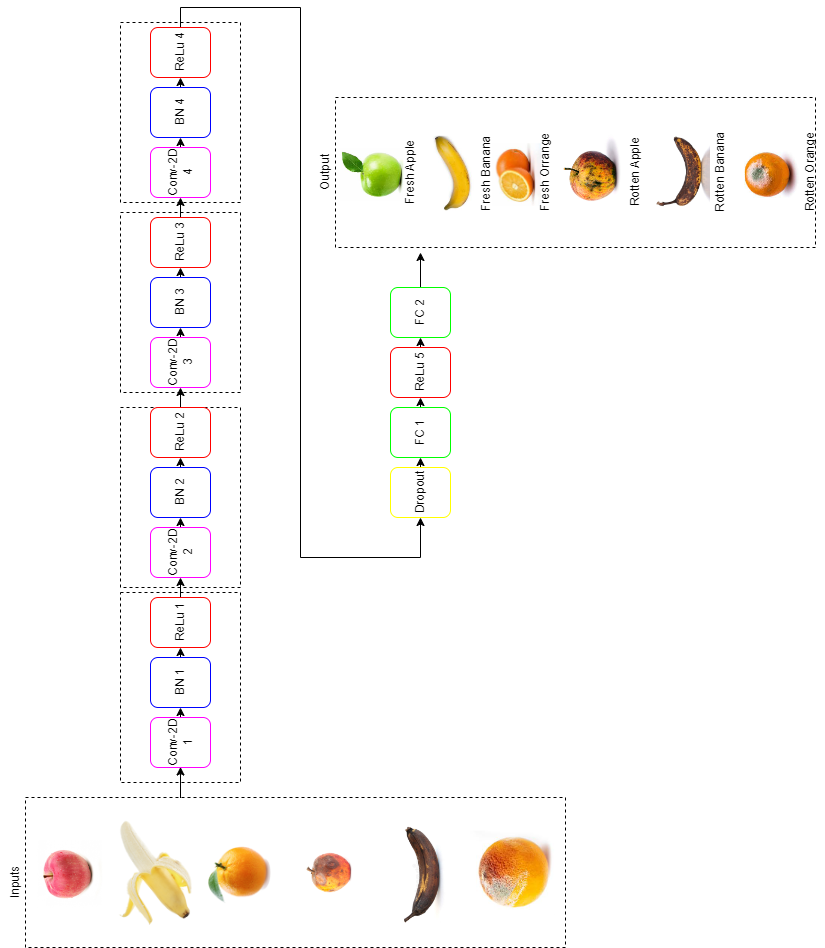
\includegraphics[width=\linewidth]{Ai Prent.drawio (1).png}
    \caption{Neural Network Architecture.}
    \label{fig}
\end{figure}

\begin{figure}[h]
    \centering
    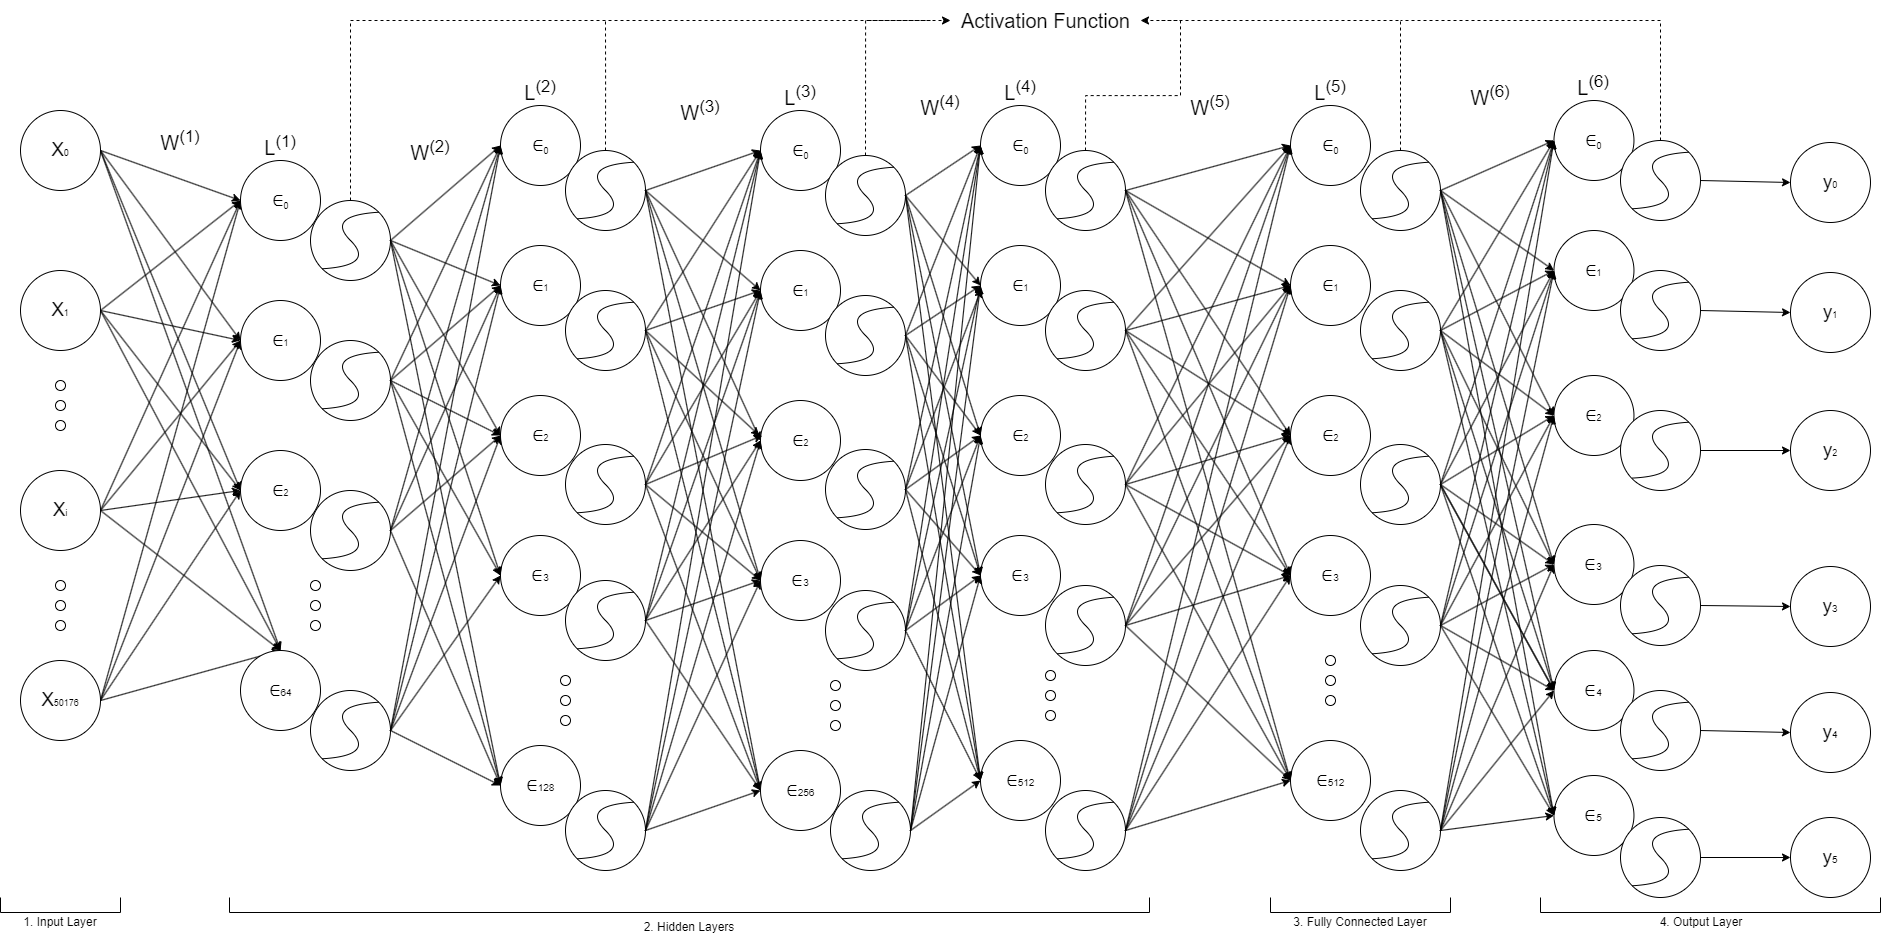
\includegraphics[width=\linewidth]{AI Architecture.drawio.png}
    \caption{Neural Network Architecture.}
    \label{fig}
\end{figure}

\subsection{Utilization of ReLU}
As ReLU, or rectified linear unit, can be effectively used in both pre-training and classification and is widely used in many applications.The structure of a deep network is complex, so it is hard to analyze the dynamics of learning process. Thus we study how complex networks need to be to approximate certain functions well. Where we optimize the trade-off between neural network complexity (measured by nonzero weights) and approximation fidelity for piecewise constant (or piecewise smooth) functions.[Analysis of Function of Rectified Linear Unit Used in Deep learning 2015]
\begin{figure}[h]
    \centering
    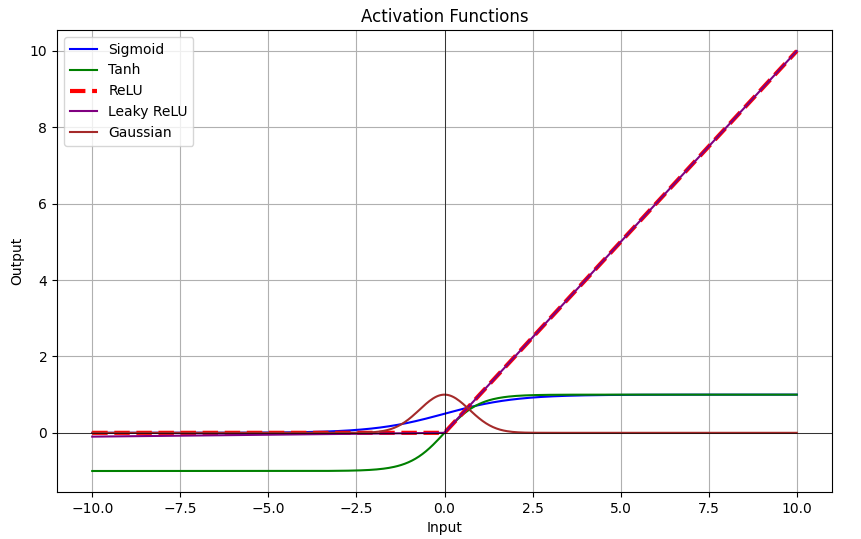
\includegraphics[width=\linewidth]{Activation Functions Compare.PNG}
    \caption{Activation Functions Comparison}
    \label{fig}
\end{figure}


\section{Training Process}

\section{Experimentation and Results}

\begin{figure}[h]
    \centering
    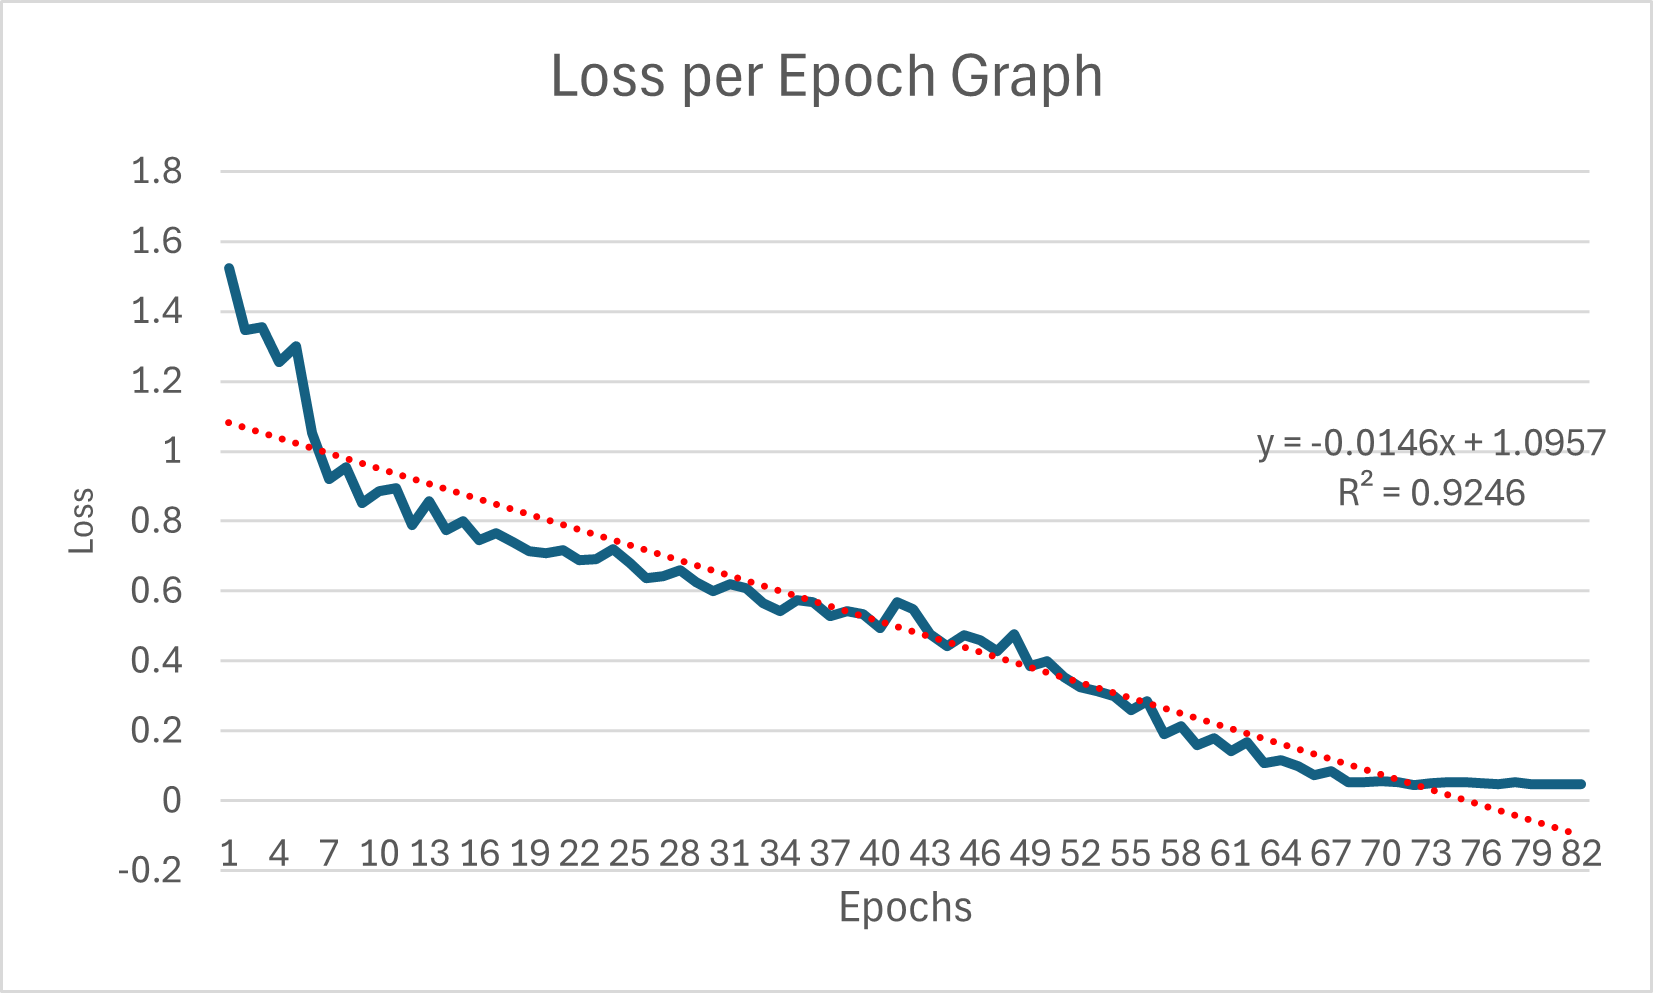
\includegraphics[width=\linewidth]{Loss_per_Epoch_Graph.png}
    \caption{Loss per Epoch.}
    \label{fig}
\end{figure}

\section{Conclusion}

\section*{Acknowledgment}

We would like to acknowledge Pieter Swanepoel for assisting us with the setup of the Google Colabe environment.

\section*{References}

Please number citations consecutively within brackets \cite{b1}. The 
sentence punctuation follows the bracket \cite{b2}. Refer simply to the reference 
number, as in \cite{b3}---do not use ``Ref. \cite{b3}'' or ``reference \cite{b3}'' except at 
the beginning of a sentence: ``Reference \cite{b3} was the first $\ldots$''

Number footnotes separately in superscripts. Place the actual footnote at 
the bottom of the column in which it was cited. Do not put footnotes in the 
abstract or reference list. Use letters for table footnotes.

Unless there are six authors or more give all authors' names; do not use 
``et al.''. Papers that have not been published, even if they have been 
submitted for publication, should be cited as ``unpublished'' \cite{b4}. Papers 
that have been accepted for publication should be cited as ``in press'' \cite{b5}. 
Capitalize only the first word in a paper title, except for proper nouns and 
element symbols.

For papers published in translation journals, please give the English 
citation first, followed by the original foreign-language citation \cite{b6}.

\begin{thebibliography}{00}
\bibitem{b1} Niculescu-Mizil, A. and Caruana, R., 2007, March. Inductive transfer for Bayesian network structure learning. In Artificial intelligence and statistics (pp. 339-346). PMLR.
\bibitem{b2} J. Clerk Maxwell, A Treatise on Electricity and Magnetism, 3rd ed., vol. 2. Oxford: Clarendon, 1892, pp.68--73.
\bibitem{b3} I. S. Jacobs and C. P. Bean, ``Fine particles, thin films and exchange anisotropy,'' in Magnetism, vol. III, G. T. Rado and H. Suhl, Eds. New York: Academic, 1963, pp. 271--350.
\bibitem{b4} K. Elissa, ``Title of paper if known,'' unpublished.
\bibitem{b5} R. Nicole, ``Title of paper with only first word capitalized,'' J. Name Stand. Abbrev., in press.
\bibitem{b6} Y. Yorozu, M. Hirano, K. Oka, and Y. Tagawa, ``Electron spectroscopy studies on magneto-optical media and plastic substrate interface,'' IEEE Transl. J. Magn. Japan, vol. 2, pp. 740--741, August 1987 [Digests 9th Annual Conf. Magnetics Japan, p. 301, 1982].
\bibitem{b7} M. Young, The Technical Writer's Handbook. Mill Valley, CA: University Science, 1989.
\end{thebibliography}

\end{document}